\documentclass{ltjsarticle}
\usepackage{luatexja}
\usepackage{amsmath}
\usepackage{graphics}
\usepackage[version=4]{mhchem}
\usepackage{siunitx}
\usepackage{graphicx}
\usepackage[top=30truemm,left=25truemm,right=25truemm]{geometry}
\title{テーマB\\接触式硫酸製造}
\author{斉藤 依緒}

\begin{document}

\section{目的!!!}
今回の実験では、工業的に重要である接触式硫酸製造を通じて反応速度・温度・平衡定数の関係について学ぶ。\\
接触式硫酸製造で用いられる酸素による二酸化硫黄の酸化は発熱反応であるため、高温であるほど平衡が反応物側にかたより、得られる生成物が少なくなる。しかし反応速度は温度と正の相関を持つため、平衡を右に偏らせようと反応温度を下げると反応速度が小さくなり、得られる生成物は少なくなる。このような問題は工業的な発熱反応では普遍的に見られ、これを防ぐために触媒が必須である。今回は温度の異なる三条件で実験を行い、反応率から平衡定数を算出することで触媒活性・化学平衡について考察する。

\section{原理}

\subsection{平衡と温度}
1で述べたように,今回の実験の反応は発熱反応である。反応式を以下に示す。

\begin{equation}
    \ce{SO2 + $\cfrac{1}{2}$O2 <=> SO3 }
\end{equation}

工業的にこの反応を行う場合、酸化バナジウム触媒(\ce{V2O4})がよく用いられる。反応の平衡定数は以下の式で表される。ここで$P_{\ce{SO2}},P_{\ce{O2}},P_{\ce{SO3}}$は平衡時の各成分の分圧を示す。

\begin{equation}
    K_p=\cfrac{[SO_3]}{[SO_2][O_2]^{1/2}}=\cfrac{P_{so_3}}{P_{SO_2}P_{o_2}^{1/2}}
\end{equation}

発熱反応においてはルシャトリエの原理より、反応温度が高くなれば温度を下げる向き、つまり吸熱反応である逆反応が支配的となる。しかし、反応速度定数は以下のアレニウスの式より反応温度が高いほど大きく、すなわち反応が早くなる。

\begin{equation}
    k=Aexp\left(-\cfrac{E_a}{RT}\right)
\end{equation}

ここで$E_a$は頻度因子と呼ばれる定数である。\\
また、熱力学的には平衡定数は以下のファントホッフの式で表される。

\begin{equation}
    \cfrac{dlnK_p}{dT}=\cfrac{\Delta H}{RT^2}
\end{equation}

ここで$\Delta H$は反応エンタルピーといい、$T=298[K]$を基準にして以下の式で表される。

\begin{equation}
    \Delta H = \Delta H_{298}^{\circ} + \int_{298}^T \Delta C_p dT
\end{equation}

また、平衡定数と温度の関係を示す実験式として、ボーデンシュタイン・ポールの式が挙げられる。

\begin{equation}
    logK_p=\cfrac{5186.3}{T} +0.611logT -6.7497
\end{equation}

今回は、(2)、(4),(6)の式をもちいてそれぞれ平衡定数を求める。

\subsection{触媒}

触媒は化学平衡には影響せず、(3)式の頻度因子に影響することで反応速度を早める働きがある。また、触媒のはたらきには温度依存性があり、ある一定以上(以下)の温度では活性を失う。\\
接触式硫酸製造に用いられる\ce{V2O4}触媒は酸化反応でよく用いられる触媒であり、珪藻土などの担体と混合して成形されることが多い。また、活性を持つ温度は410℃~580℃の間である。工業的な反応の設計においては、平衡温度・反応速度の温度依存に加え、触媒が活性を持つ温度を設定しなくてはならない。

\section{方法}

\subsection{試薬}

今回用いた試薬を以下に示す。\\
《硫酸製造》

\begin{itemize}
    \item \ce{H2SO4}(工業用濃硫酸)\ :2L
    \item (一級試薬500g)\ :1本
    \item \ce{V2O5}触媒\ :1本
    \item \ce{CaCl2}(U字管乾燥用)\ :1本
    \item 0.05[M] \ce{I2}水溶液\ :50mL
\end{itemize}

《\ce{SO3}滴定》

\begin{itemize}
    \item でんぷん水溶液\ :2,3滴
    \item 0.1[M]\ce{Na2S2O3}水溶液
\end{itemize}

《\ce{SO2}滴定》

\begin{itemize}
    \item 3\% \ce{H2O2}水溶液\ :10mL
    \item 0.1[M] \ce{NaOH}水溶液
    \item メチルレッド\ :2,3滴
\end{itemize}

\subsection{実験器具・装置}

《滴定用器具》

\begin{itemize}
    \item ビュレット(50[$cm^3$])
    \item ホールピペット(50,25、10$[cm^3]$)
    \item ビーカー(1L,50,30$[cm^3]$)
    \item 三角フラスコ(200$[cm^3]$)
    \item \ce{SO2}吸収瓶
    \item \ce{SO3}吸収瓶
    \item シリンジ
\end{itemize}

《実験装置》\\

今回の接触式硫酸製造には以下のような装置を用いる。\\
まず、空気はコンプレッサーで圧縮されたのち、\ce{CaCl2}管、濃硫酸によって乾燥される。同様に、\ce{SO2}も乾燥したのち、転化器手前の混合瓶で混合される。混合瓶から反応器の間には三方コックがあり、ここで流路を変えてガス採集瓶に反応前のガスを溜めることができる。また、ガス採集瓶の体積は514mLである。転化器は\ce{V2O5}触媒で満たされており、混合ガスは固体触媒の隙間を通りながら反応する。\\
また、転化器には熱電対・温度制御器が接続されており、反応温度を一定に保つことができる。\\
転化器の後にも三方コックが接続されている。片方は濃硫酸入りフラスコ・もう片方は\ce{SO3}採集瓶と\ce{I2}水溶液フラスコが直列に接続されている。反応初期では十分な反応が起こらず、触媒表面の\ce{SO3}と水蒸気が反応して不純物である硫酸が発生するため、流路を濃硫酸がわに設定して混入を避ける。\\

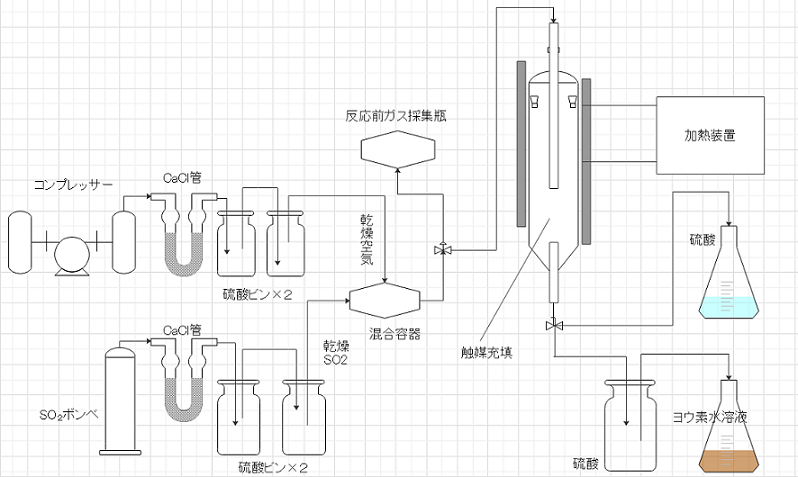
\includegraphics[width=8cm]{反応装置図.png}

\subsection{実験方法}

今回の実験は、\ce{SO3}生成・\ce{I2}滴定・\ce{SO2}滴定の3つの部分に分かれている。これらの実験を反応温度400℃,500℃,600℃の三回行った。

\subsubsection{\ce{SO3}生成}

\begin{enumerate}
    \item 反応器に接続する前の\ce{SO3}採集瓶(硫酸を充填してあるもの)の質量を測定した。
    \item \ce{I2}水溶液を\ce{so2}採集フラスコ内に充填した。このとき、濃度が変わらないよう、使用するホールピペットは共洗いを行った。また、ガスが溶液に泡状となって直接吹き込まれる(この状態をバブリングという)よう、イオン交換水で体積を調整した。
    \item 反応器の前に接続されている三方コックで流路を切り替え、反応前ガスを採集した。
    \item 吸収瓶などをバネで接続し、反応前ガスを流入させて反応を開始した。このとき、反応初期段階のガスは採集せずに濃硫酸に回収し、反応が十分に進んでから流路を切り替えた。
    \item 反応終了後、\ce{SO3}採集瓶の質量を測定した。
\end{enumerate}

\subsubsection{\ce{I2}滴定}

\ce{SO3}反応後、生成物に混入した\ce{SO2}は以下の式のように\ce{I2}を還元する。

\begin{equation}
    \ce{I2 + SO2 + 2H2O -> 2HI + H2SO4}
\end{equation}

そのため、還元されずに残存した\ce{I2}の物質量から未反応\ce{SO2}の物質量を求めるため、\ce{I2}濃度を測定する滴定を行った。この滴定は以下の\ce{S2O3^{2-}}イオンが\ce{I2}を還元する反応を利用している。

\begin{equation}
    \ce{I2 + 2S2O3^{2-} -> 2I^- + S4O6^{2-}}
\end{equation}

また、\ce{I2}滴定の大まかな手順を以下のフローチャートに示す。\\
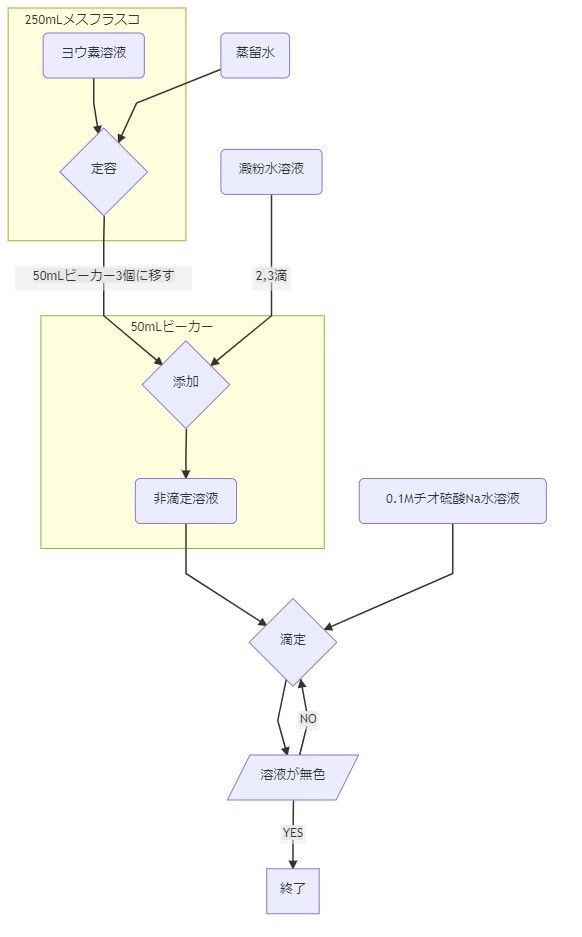
\includegraphics[width=8cm]{ヨウ素滴定.jpg}

\begin{enumerate}
    \item \ce{SO3}生成反応後 、\ce{SO2}を吸収した\ce{i2}水溶液を250mLメスフラスコに開けた。このとき、使用したガラス管・三角フラスコ・漏斗をすべて蒸留水で洗浄し、洗浄液もメスフラスコに移した。
    \item メスフラスコの標線まで蒸留水を足して定容し、蓋をしてよく攪拌した。
    \item 50mLずつビーカーに移し、澱粉水溶液を2,3滴加え、これを非滴定溶液とした。同じものを3個作成した。
    \item それぞれの非滴定溶液を0.1Mの\ce{Na2S2O3}水溶液で非滴定溶液が無色透明になるまで滴定した。滴定は三回行い、三回の平均値を滴定に要した\ce{Na2S2O3}の体積とした。
\end{enumerate}

\subsubsection{\ce{SO2}滴定}

転化率を算出するため、反応前ガスの\ce{SO2}濃度を知る必要がある。今回は、採集瓶に採取したガス中の\ce{SO2}を\ce{H2O2}で還元し、\ce{H2SO4}とした。これを塩基である\ce{NaOH}で中和することで滴定を行い、\ce{SO2}濃度を測定した。

\begin{equation}
    \ce{SO2 + H2O2 -> H2SO4}
\end{equation}

\begin{equation}
    \ce{H2SO4 + OH^- -> H2O + HSO4^- }
\end{equation}

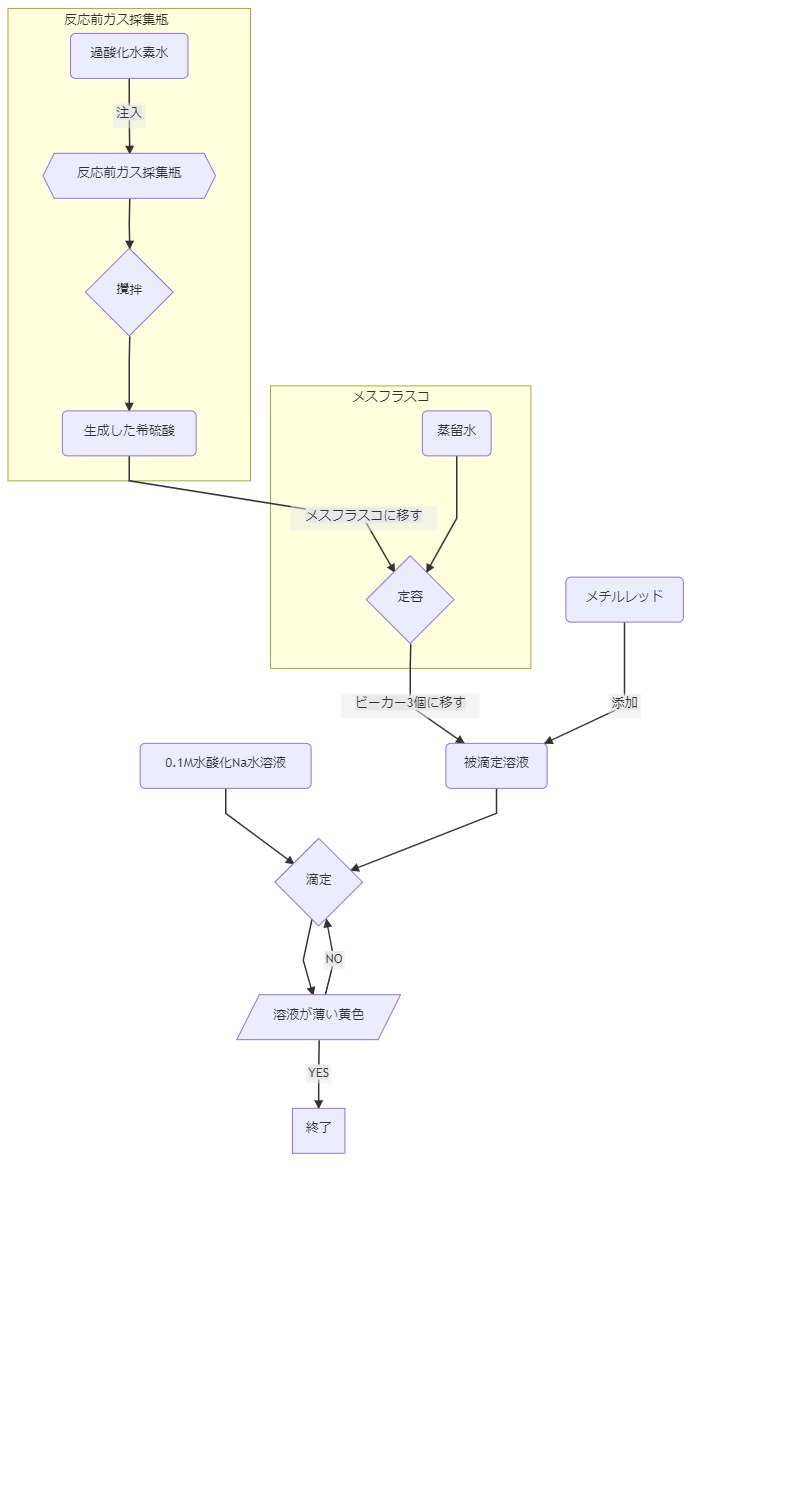
\includegraphics[width=8cm]{硫酸滴定.jpg}
\begin{enumerate}
    \item 反応装置に接続していた水銀マノメーターから、反応装置の内圧を読み取った。
    \item 反応前ガス採集瓶にシリンジで\ce{H2O2}水溶液を10mL注入し、良く振って攪拌することで\ce{SO2}を反応させた。
    \item 採集瓶中の溶液を100mLメスフラスコに移し、定容した。この時、採集瓶中に溶液がのこらないよう、共洗いを行った。
    \item メスフラスコを良く振ったのち、溶液を3個のビーカーに25mLずつ採取し、それぞれにメチルレッドを2,3滴ずつ加えて被滴定液とした。
    \item 被滴定液を0.1Mの\ce{NaOH}水溶液で溶液が薄い黄色になるまで滴定した。滴定は三回行い、平均値を滴定に要した\ce{NaOH}体積とした。
\end{enumerate}


\section{結果}

\subsection{式の導出}

今回の反応の平衡定数$K_p$は(2)式で表される。\\
また、\ce{SO2}から\ce{SO3}への転化率xは以下の式で表される。

\begin{equation}
    x=\cfrac{\ce{SO3}の物質量}{\ce{SO2}の物質量+\ce{SO3}の物質量}
\end{equation}

(11)式より、以下のことが言える。

\begin{equation}
    1-x =\cfrac{\ce{SO2}の物質量}{\ce{SO2}の物質量+\ce{SO3}の物質量}
\end{equation}

反応前ガスの\ce{SO2}濃度をa[vol\%],\ce{O2}濃度をb[vol\%],反応器の内圧をP[atm]とする。\\
(11),(12)式より、平衡時の\ce{SO2},\ce{SO3}の物質量比は以下のようになる。

\begin{equation}
    \cfrac{\ce{SO3}物質量}{\ce{SO2}物質量}=\cfrac{x}{1-x}
\end{equation}

また、\ce{O2}物質量を考えるため、ガス全体の物質収支を取る。\\

\begin{table}[htb]
    \caption{物質収支}
    \begin{center}
        \begin{tabular}{|c|c|c|c|c|}\hline
            状態   & \ce{SO2} & \ce{O2}           & \ce{SO3} & 合計                \\  \hline
            反応前 & a        & b                 & 0        & a+b                 \\ \hline
            増減   & -ax      & $-\cfrac{ax}{2}$  & +ax      & $-\cfrac{ax}{2}$    \\ \hline
            反応後 & a(1-x)   & $b-\cfrac{ax}{2}$ & ax       & $a+b-\cfrac{ax}{2}$ \\ \hline
        \end{tabular}
    \end{center}
\end{table}

反応器内圧Pを考えれば、反応器中の\ce{O2}分圧は以下の式で表される。

\begin{equation}
    P_{\ce{O2}}=\cfrac{b-\cfrac{ax}{2}}{100-\cfrac{ax}{2}}\cdot P
\end{equation}

(13),(14)式を(2)式に代入し、以下の式を得る。

\begin{equation}
    K_p=\cfrac{P_{\ce{SO3}}}{P_{\ce{SO2}}P_{\ce{O2}}^{1/2}}=\cfrac{x}{1-x}\cdot\cfrac{1}{\sqrt{\cfrac{b-\cfrac{ax}{2}}{100-\cfrac{ax}{2}}\cdot P}}
\end{equation}

\subsection{測定結果}
\subsubsection{\ce{SO3}生成反応}
400℃,500℃,600℃の各温度について、\ce{SO3}質量(反応前後の採集瓶の質量差)・\ce{SO3}物質量を以下の表2に示す。

\begin{table}[htb]
    \caption{\ce{SO3}生成}
    \begin{center}
        \begin{tabular}{|c|c|c|}\hline
            温度[℃] & \ce{SO3}質量[g] & 物質量[mol]            \\  \hline\hline
            400     & 0.31            & $3.87 \times 10^{-3}$  \\ \hline
            500     & 0.93            & $11.6 \times 10^{-3} $ \\ \hline
            600     & 0.35            & $4.37 \times 10^{-3} $ \\ \hline
        \end{tabular}
    \end{center}
\end{table}

\subsubsection{\ce{I2}滴定}
400 ℃,500℃,600℃の各温度について、滴定に要した\ce{Na2S2O3}体積(三回の試行の平均値)平均),非滴定液50mL中の残存\ce{I2}物質量,250mL中の残存\ce{I2}物質量,吸収された\ce{SO2}物質量を以下の表にしめす。(7),(8)式より、\ce{I2}一分子を還元するのに\ce{Na2S2O3}は二分子,\ce{SO2}は一分子必要である。また、\ce{I2},\ce{Na2S2O3}それぞれの活量係数として1.003,1.004を用い、有効数字三桁で算出した。

\begin{table}[htb]
    \caption{\ce{I2}滴定}
    \begin{center}
        \begin{tabular}{|c|c|c|c|c|}\hline
            温度[℃] & \ce{Na2S2O3}体積[mL] & 50mL中残存\ce{I2}[mol]  & 250mL中残存\ce{I2}[mol] & \ce{SO2}吸収量[mol]   \\  \hline\hline
            400     & 3.76                 & $0.188 \times 10^{-3}$  & $0.940 \times 10^{-3}$  & $1.56 \times 10^{-3}$ \\ \hline
            500     & 5.01                 & $0.251 \times 10^{-3} $ & $1.25 \times 10^{-3}$   & $1.25 \times 10^{-3}$ \\ \hline
            600     & 3.86                 & $0.193 \times 10^{-3} $ & $0.965 \times 10^{-3}$  & $1.54 \times 10^{-3}$ \\ \hline
        \end{tabular}
    \end{center}
\end{table}

\subsubsection{\ce{NaOH}滴定}

各温度における反応前のガスについて、滴定に要した\ce{NaOH}体積(三回の平均値)、非滴定液25mL中に含まれていた\ce{SO2}物質量,ガス採集瓶(体積514mL)中に含まれていた\ce{SO2}物質量を以下に示す。滴定に用いた\ce{NaOH}の活量係数は1.005である。

\begin{table}[htb]
    \caption{\ce{NaOH}滴定}
    \begin{center}
        \begin{tabular}{|c|c|c|c|}\hline
            反応温度[℃] & \ce{NaOH}体積[mL] & 25mL中\ce{SO2}[mol]     & 採集瓶中\ce{SO2}[mol]  \\  \hline\hline
            400         & 9.82              & $0.987 \times 10^{-3}$  & $3.95 \times 10^{-3}$  \\ \hline
            500         & 10.52             & $1.057 \times 10^{-3} $ & $4.228 \times 10^{-3}$ \\ \hline
            600         & 11.23             & $1.129 \times 10^{-3} $ & $4.514 \times 10^{-3}$ \\ \hline
        \end{tabular}
    \end{center}
\end{table}

\subsubsection{反応前ガス組成・転化率算出}

各温度について、反応前ガス温度,反応器内圧,入口ガス中\ce{SO2}濃度[vol\%]a,入口ガス中\ce{O2}濃度[vol\%]b,転化率xを以下の表4に示す。入口ガス中\ce{SO2}濃度は理想気体の状態方程式を用い、\ce{SO2}が占める体積を求めることで算出した。この時気体定数$R=0.082[(L\cdot atm)/(K \cdot mol)]$を用いた。また、転化率は(11)式により算出した。

\begin{equation}
    V_{\ce{SO2}}=\cfrac{n_{\ce{SO2}}RT}{P}
\end{equation}

\begin{equation}
    a=\cfrac{V_{\ce{SO2}}}{V}
\end{equation}

また、入口ガス中\ce{O2}濃度bは、\ce{SO2}濃度aより以下の式で求められる。

\begin{equation}
    b=0.209(100-a)
\end{equation}

\begin{table}[htb]
    \caption{\ce{NaOH}滴定}
    \begin{center}
        \begin{tabular}{|c|c|c|c|c|c|}\hline
            反応温度[℃] & 反応前ガス温度[℃] & 内圧[atm] & \ce{SO2}濃度[vol\%]a & \ce{O2}濃度[vol\%]b & 転化率x \\  \hline\hline
            400         & 25.3              & 0.996     & 18.9                 & 17.0                & 0.713    \\ \hline
            500         & 23.1              & 0.998     & 20.0                 & 16.7                & 0.903    \\ \hline
            600         & 25.3              & 0.996     & 21.6                 & 16.4                & 0.740    \\ \hline
        \end{tabular}
    \end{center}
\end{table}

\subsection{平衡定数算出}
(15)式、(5)の熱力学的理論平衡定数の式、(6)のボーデンシュタイン・ポールの式を用い、各温度の平衡定数を算出した。結果を以下の表に示す。また、これらの
値を$1/T$に対しプロットしたグラフを図に示す。

\begin{table}[htb]
    \caption{平衡定数}
    \begin{center}
        \begin{tabular}{|c|c|c|c|}\hline
            反応温度[℃] & 平衡定数(実験値) & 熱力学的平衡定数 & ボーデンシュタイン・ポールの平衡定数 \\  \hline\hline
            400         & 7.52             & 583              & 483                                  \\ \hline
            500         & 32.1             & 64.9             & 53.0                                 \\ \hline
            600         & 9.44             & 12.5             & 9.73                                 \\ \hline
        \end{tabular}
    \end{center}
\end{table}

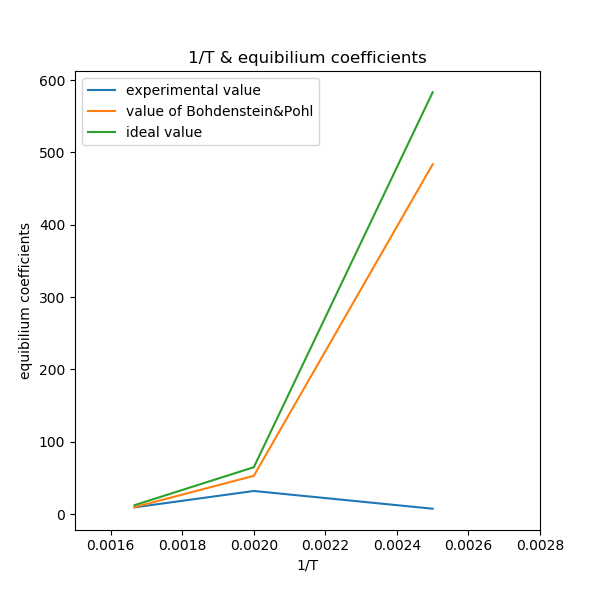
\includegraphics[width=8cm]{Figure_1.png}

\section{考察}
\subsection{各温度における平衡定数の考察}

得られた平衡定数について、温度ごとに考察する。\\
《400℃》\\
この反応は発熱反応であるため、低温ほど平衡定数が大きくなる。ゆえに理論平衡定数・ボーデンシュタイン・ポールの式の平衡定数は3条件のなかで最も大きい値が得られた。しかし、実験により求めた平衡定数はこれらの値を大きく下回る。これは、反応温度が低いために反応速度が小さく、短時間の実験では定常状態に達していなかったことが原因であると考える。今回用いた\ce{V2O5}触媒は反応温度が約410℃を超えないと活性が発現しないため、触媒による反応速度の増大もおこらなかったと推測される。ゆえに、この条件での反応は平衡に達していなかったため、平衡定数が小さかったと考える。\\
\\
《500℃》\\
500℃においても理論平衡定数・ボーデンシュタイン・ポールの平衡定数よりも小さい値が得られたが、400℃と比較すると差は小さく、約20~30の差におさまった。また、実験値どうしを比較すると、3条件のなかで最も平衡定数・転化率ともに大きい値が得られた。500℃は\ce{V2O5}触媒が使用可能な温度の範囲内であることから、比較的早く平衡状態に達すると考えられる。また、反応が発熱反応であり、触媒によって反応速度が大きくなっていることから反応器内の温度は500℃よりも高くなっており、平衡も500℃のときと比較して左(反応物側)にずれていたと推察される。そのため、この温度で得られた平衡定数は正確には500℃での平衡定数ではなかったと考える。\\
\\
《600℃》\\
この温度条件で得られた平衡定数は理論値と最も近い値であった。\ce{V2O5}触媒は580℃ほどで活性を失うが、600℃においては平衡が左にかたよっており、高温で反応速度も大きい。このことから、触媒の活性が無かったとしても実験時間中に平衡に達したため、理論平衡定数と近い値が得られたと考える。\\理論反応定数との差異は500℃における実験同様、反応器内の温度が発熱反応により上昇していたと考える。

\subsection{転化率を上げるには}

今回の実験では、反応温度500℃の際に最も高い転化率が得られた。\\
これは、500℃のときに触媒活性があり、平衡に近い状態に達するまでの時間と平衡定数による理論収率のバランスが最もよかったためと考えられる。しかし、この反応の平衡定数・理論収率は課題にて後述するが低温ほど大きくなる。ゆえに低温下で活性を持つ触媒を用い、転化器内の排熱が効率的に行われればさらに高い転化率が期待できる。また、ルシャトリエの原理を考慮すると、反応後ガス(未反応\ce{SO2},\ce{O2},反応により生成した\ce{SO3}の混合物)から\ce{SO3}を選択的に取り除くことができれば平衡は右に偏ると考えられる。\\また、転化器内でのガスの滞在時間を長くすることができれば、反応時間が長くなり理論転化率に近づけることが可能である。\ce{SO2}は空気よりも比重が大きいため、反応前ガスも反応器内で重力の影響を受け、ガスの滞在時間が短くなっている可能性がある。ゆえに、反応器を横向きに設計したときに転化率が上昇する可能性があると考える。

\section{課題}
\ce{SO2}10[vol\%],\ce{O2}18[vol\%],\ce{N2}72[vol\%]のガスについて、理論転化率を以下の表に示す。

\begin{table}[htb]
    \caption{理論転化率}
    \begin{center}
        \begin{tabular}{|c|c|c|}\hline
            反応温度[℃] & 転化率x & 平衡定数 \\  \hline\hline
            400         & 0.995    & 583      \\ \hline
            500         & 0.960    & 64.9     \\ \hline
            600         & 0.826    & 12.5     \\ \hline
        \end{tabular}
    \end{center}
\end{table}

\section{参考文献}
\begin{itemize}
    \item アトキンス物理化学(上)第10版 2017/3/10 (訳)中野元祐 東京化学同人発行
    \item 『需給拡大する硫酸工業の現状と未来』 化学と教育61巻9号 2013年 須藤実
    \item 接触硫酸製造用ヴアナジウム触媒の性能向上に関する研究(第1報:触媒の活性変化について 北海道大學工學部研究報告, 12, 127-138 1955/6/15 岡本剛,小林晴夫,石井忠雄,小田中秀雄
\end{itemize}

\end{document}